\documentclass[UTF8,zihao=-4]{ctexart}
\usepackage{graphicx}
\usepackage[a4paper, margin=2cm, top=2.5cm, bottom=2.5cm]{geometry}
\usepackage{enumitem}
\usepackage{amsmath}
\usepackage{amssymb}
\usepackage{xcolor}
\definecolor{sectionblue}{rgb}{0.1, 0.3, 0.6}
\usepackage{titlesec}
 \usepackage{float}
% --- 自定义格式，使其更像一份正式的报告 ---
\setlist{nosep, leftmargin=*}
\linespread{1.3}
\titleformat{\section}{\Large\bfseries\color{sectionblue}}{\thesection}{1em}{}
\titleformat{\subsection}{\large\bfseries}{\thesubsection}{1em}{}
\titleformat{\subsubsection}{\bfseries}{\thesubsubsection}{1em}{}

\newcommand{\keyterm}[1]{\textit{\textcolor{blue}{#1}}}

\title{\Huge\bfseries 论文大纲}
\author{Dongming Li}
%\date{\today}

\begin{document}

\maketitle
\thispagestyle{empty}
\newpage
\tableofcontents
\newpage

% ===================================================================
\section{摘要 (Abstract) - 研究成果的高度凝练}
% ===================================================================
\begin{itemize}
    \item \textbf{宏观挑战：} 植入式医疗设备（IMDs）正向分布式网络演进，这要求通信系统必须在动态、甚至病理性的生物环境中保持超低功耗与高鲁棒性。
    \item \textbf{具体问题定义：} 多腔无导线起搏器（LCPs）的心内通信（CIC）是此领域的极限挑战。其信道特性具有双重复杂性：1) 健康心律下的\keyterm{周期性波动}；2) 房室传导阻滞等病理状态下的\keyterm{非周期性、不可预测的深度衰落}。
    \item \textbf{本文方案与核心创新：} 提出了一种基于超再生接收机（SRR）的自适应接收架构。其核心是一种\keyterm{无需外部心电图（ECG）信号}的混合信号自动增益控制（AGC）系统。该系统的关键创新在于一个心跳同步的\keyterm{双自由度（2-DOF）控制策略}：
        \begin{itemize}
            \item \textbf{预测前馈 (Predictive Feedforward):} 利用每个心跳的峰值接收信号强度指示（RSSI）作为心脏机械节律的代理，\textit{主动预测}并\textit{前瞻性补偿}由病理事件引发的非周期性阶跃干扰。
            \item \textbf{增量式反馈 (Incremental Feedback):} 通过一个PID控制器，\textit{实时校正}心跳内的周期性波动和预测模型的残余误差。
        \end{itemize}
    \item \textbf{严谨的验证方法学：} 构建了一套\keyterm{双路径定量评估框架}。该框架以一个可编程的\keyterm{高保真度离体猪心灌注平台}为核心，用于在可复现的病理动态下进行端到端链路性能评估；同时辅以\keyterm{硬件在环（HIL）仿真}，对控制器的瞬态响应特性进行精确表征。
    \item \textbf{定量化的核心成果：} 实验结果表明，所提出的2-DOF控制器能在超过15\,dB的信道波动下，将输入信号稳定在目标值的1\%以内。这一高稳定性最终转化为通信性能的巨大飞跃，实现了误码率（BER）近两个数量级的降低，在5\,kbps数据率下性能提升因子超过\textbf{60倍}。
    \item \textbf{科学与工程意义：} 本研究不仅为临床可靠的LCPs系统提供了一项关键使能技术，更重要的是，为下一代旨在严苛生物环境中稳健运行的网络化IMDs，提供了一套经过系统性验证的、可推广的\keyterm{自适应通信设计范式}。
\end{itemize}

% ===================================================================
\section{引言 (Introduction)}
% ===================================================================
\subsection{宏观背景：植入式医疗设备的范式转变}
\begin{itemize}
    \item \textbf{技术演进路径：} 从“功能孤岛”到“分布式协作网络”。IMDs不再是独立的感知或治疗单元，而是演变为协同工作的“体内网络”（In-Body Networks），以实现更复杂的诊断与治疗策略。
    \item \textbf{核心技术瓶颈的显现：} 这一转变的实现，高度依赖于在人体这一 perpetually dynamic （永远动态）的生物媒介内，建立长期、稳定、且符合微瓦级功耗预算的无线通信链路。这构成了该领域的核心技术瓶颈。
\end{itemize}

\subsection{技术选型分析：现有无线技术的局限性与GCC的优势}
\begin{itemize}
    \item \textbf{现有技术评估：} 对传统无线方案进行系统性评估，指出其在人体环境下的固有缺陷：
        \begin{itemize}
            \item \textbf{射频 (RF):} 组织吸收导致的高路径损耗 $\rightarrow$ 高发射功率需求 $\rightarrow$ 与IMDs的能量预算不兼容。
            \item \textbf{磁感应耦合:} 工作范围受限于近场 $\rightarrow$ 严格的距离与对准要求 $\rightarrow$ 不适用于位置可能变化的腔内设备。
            \item \textbf{超声波:} 高方向性 $\rightarrow$ 依赖直瞄链路（Line-of-Sight） $\rightarrow$ 在器官遮挡和多路径环境中可靠性差。
        \end{itemize}
    \item \textbf{新兴方案的确立：} 人体信道通信（Galvanic Conductive Communication, GCC）利用人体组织的导电性传输微弱电流信号。
        \begin{itemize}
            \item \textbf{核心优势：} 1) 信号被天然约束在体内，安全性高；2) 传输功耗极低；3) 电路实现相对简单。这些特性使其成为下一代网络化IMDs的理想候选技术。222
        \end{itemize}
\end{itemize}

\subsection{研究问题的聚焦：以多腔起搏器为极限测试场景}
\begin{itemize}
    \item \textbf{确定研究载体：} 在所有GCC应用场景中，多腔无导线起搏器（LCPs）的心内通信环境最为复杂和严苛，因此被选定为检验GCC技术稳健性的\keyterm{极限测试场景 (corner case)}。
    \item \textbf{识别文献空白：} 指出现有关于CIC信道的研究，大多基于\keyterm{静态或准静态模型}，这些模型简化或平均了心脏机电活动的影响，未能捕捉到信道的真实动态特性，从而限制了现有收发机设计的临床可靠性。
\end{itemize}

\subsection{核心科学问题：心内信道双重动态特性的解构}
\label{sec:core_problem}
本研究的立论基础，在于首次清晰地将心内信道的动态性解构为两个性质完全不同的层面。这两个层面共同对通信链路的稳定性构成了根本性威胁，且需要不同的策略来应对。

\subsubsection{第一重挑战：健康节律下的“周期性”信道波动 (可预测的干扰)}
\begin{itemize}
    \item \textbf{物理机制：} 在正常窦性心律下，心肌的等容收缩/舒张和快速射血/充盈阶段，导致心腔的几何形态和腔内血液的电导率发生规律性的、与心动周期同步的变化。
    \item \textbf{对通信的影响：} 这种变化直接调制了收发电机极间的传输路径，引起信道增益出现高达10-15dB的\keyterm{周期性、可预测的}波动。
    \item \textbf{对策的必然性：} 这一基线动态特性本身，就排除了静态接收机方案的可能性，并确立了\keyterm{自动增益控制（AGC）}作为维持通信质量的\textbf{基础性技术前提}。
\end{itemize}
\begin{figure}[H]
    \centering
    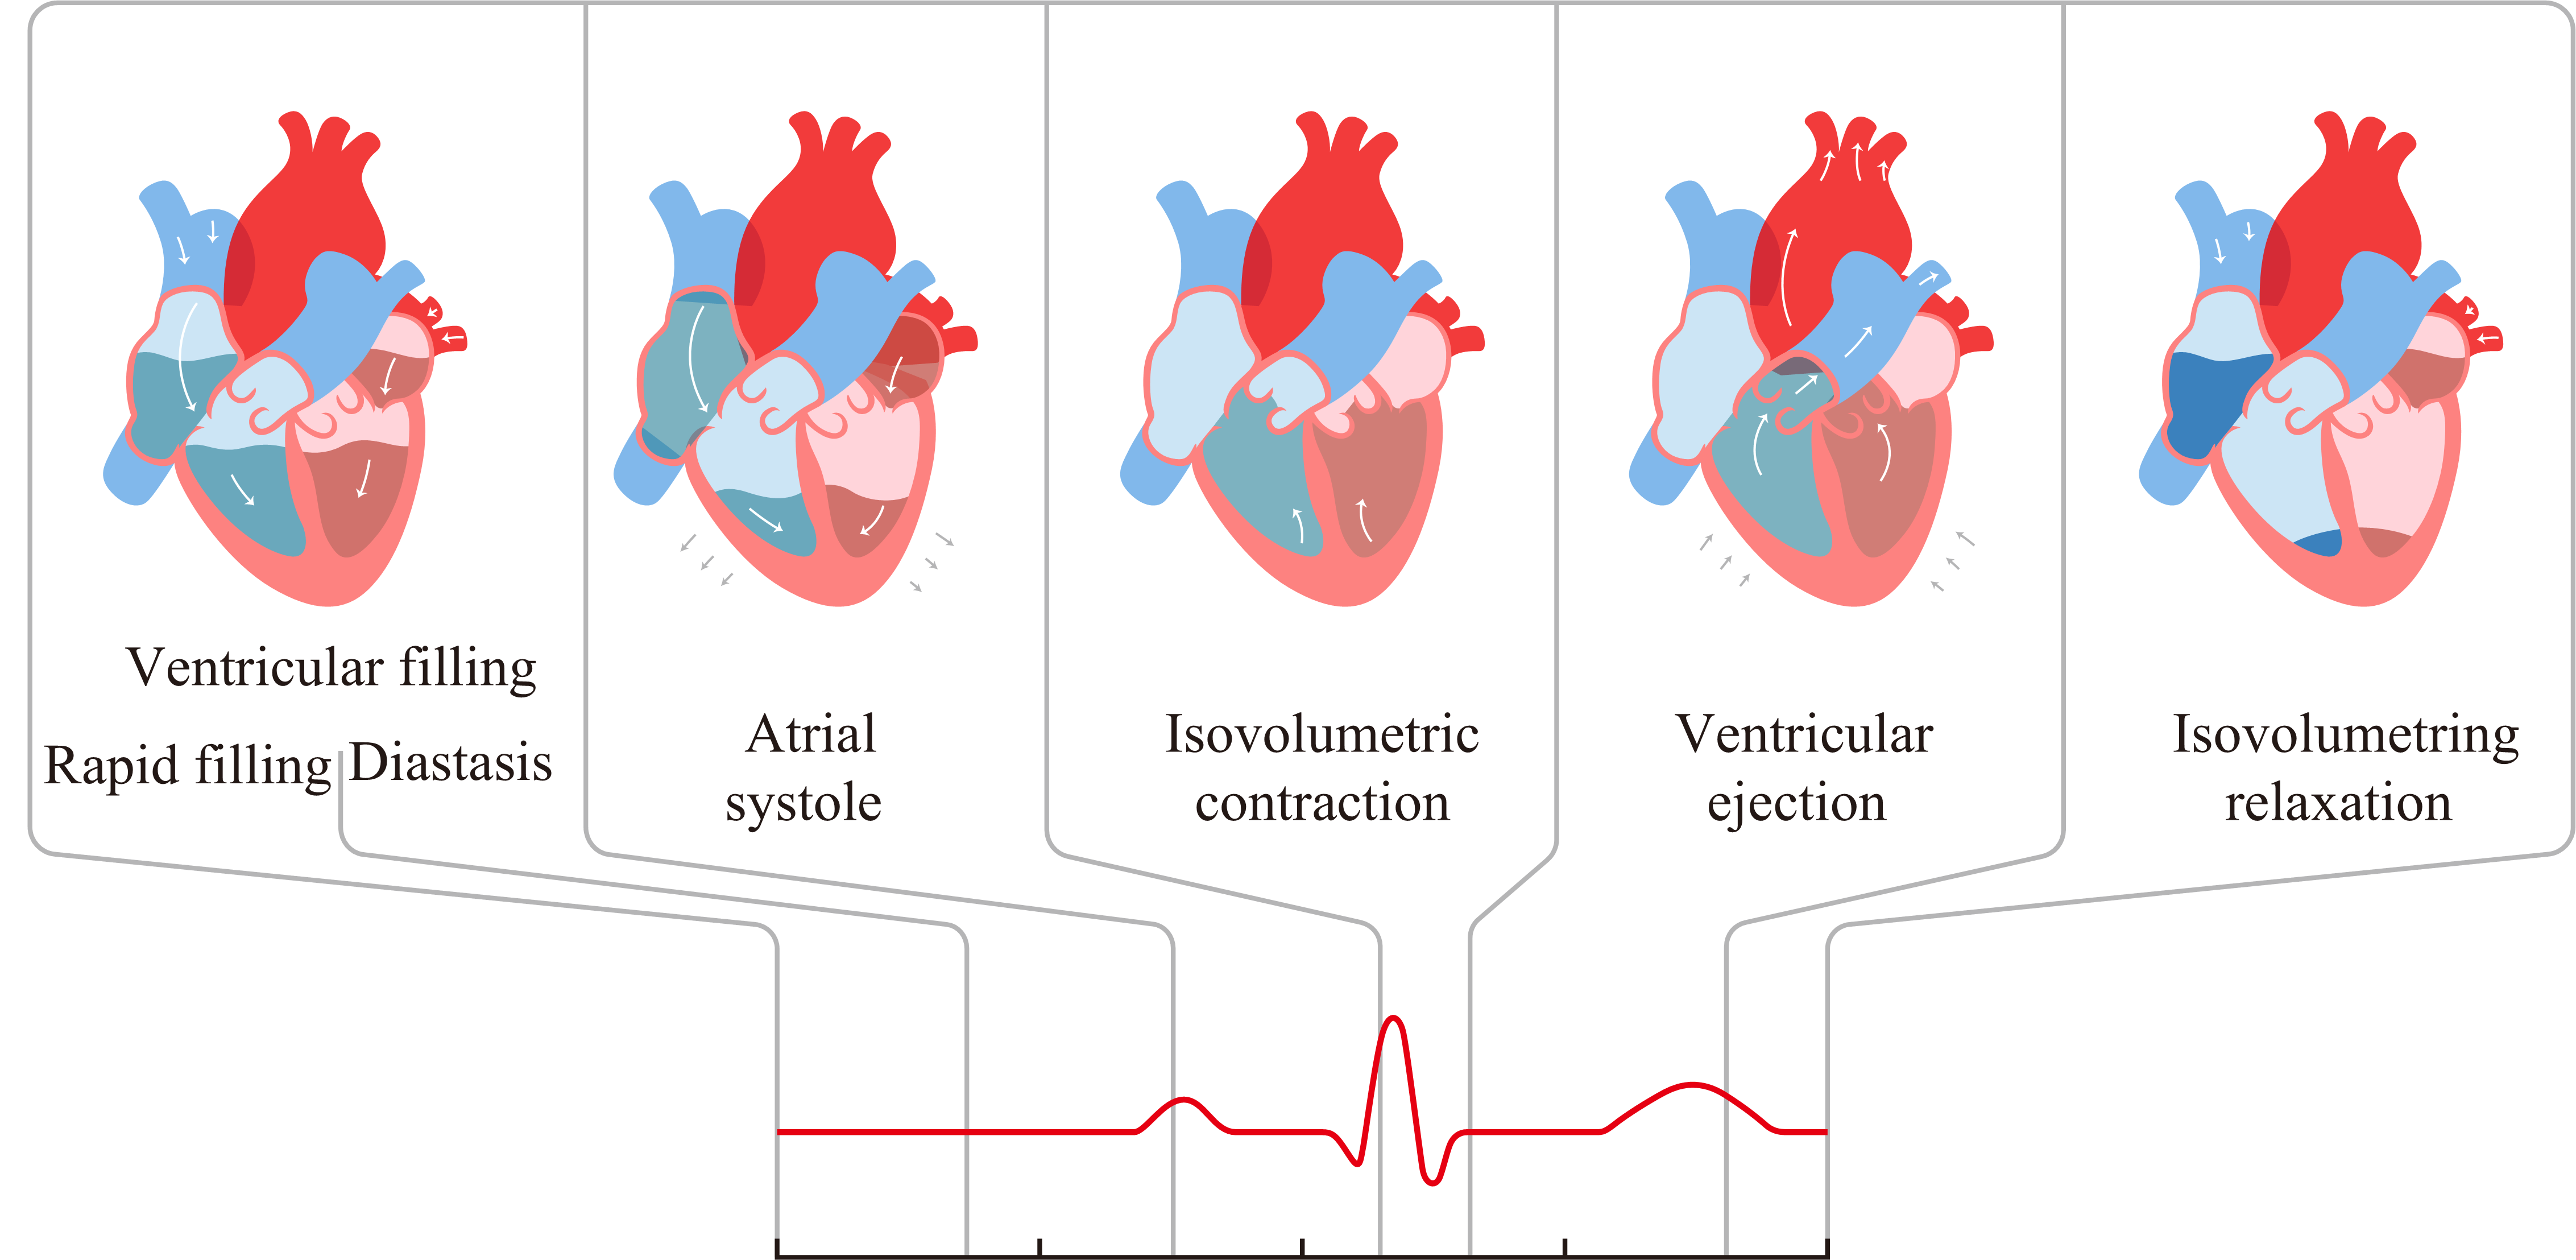
\includegraphics[width=0.7\linewidth]{Figure/cycle.png}
    \caption{图解第一重挑战：健康心动周期中，ECG电活动与心室容积变化（代表信道变化）之间的规律性与可预测性。}
\end{figure}

\subsubsection{第二重挑战：病理节律下的“非周期性”信道衰落 (不可预测的灾变)}
\begin{itemize}
    \item \textbf{临床现实：} LCPs的主要应用对象是心律失常患者。在如“房室传导阻滞”等临床病理条件下，心脏的传导系统会间歇性失效，导致心跳“漏搏”。
    \item \textbf{对通信的影响：} 这种事件打破了原有的心动周期，导致信道增益出现\keyterm{非周期的、突发的、更深度的}衰落。这种衰落是\keyterm{不可预测的灾变性事件}。
    \item \textbf{传统方案的失效：} 传统的、纯粹基于反馈的AGC机制（如常规PID），其工作原理是“检测到误差后再进行补偿”。其固有的\keyterm{响应延迟}使其在面对此类突发事件时，必然会经历一个信号大幅偏离目标的“失锁”窗口，导致瞬时通信中断。这构成了将原型设备推向临床应用的\textbf{根本性障碍}。
    \item \textbf{引出本文核心目标：} 因此，本研究的核心科学问题是：如何设计一种能够超越传统“事后”补偿的智能AGC，以实现对信道突变的\keyterm{主动预测与前瞻性补偿}。
\end{itemize}
\begin{figure}[H]
    \centering
    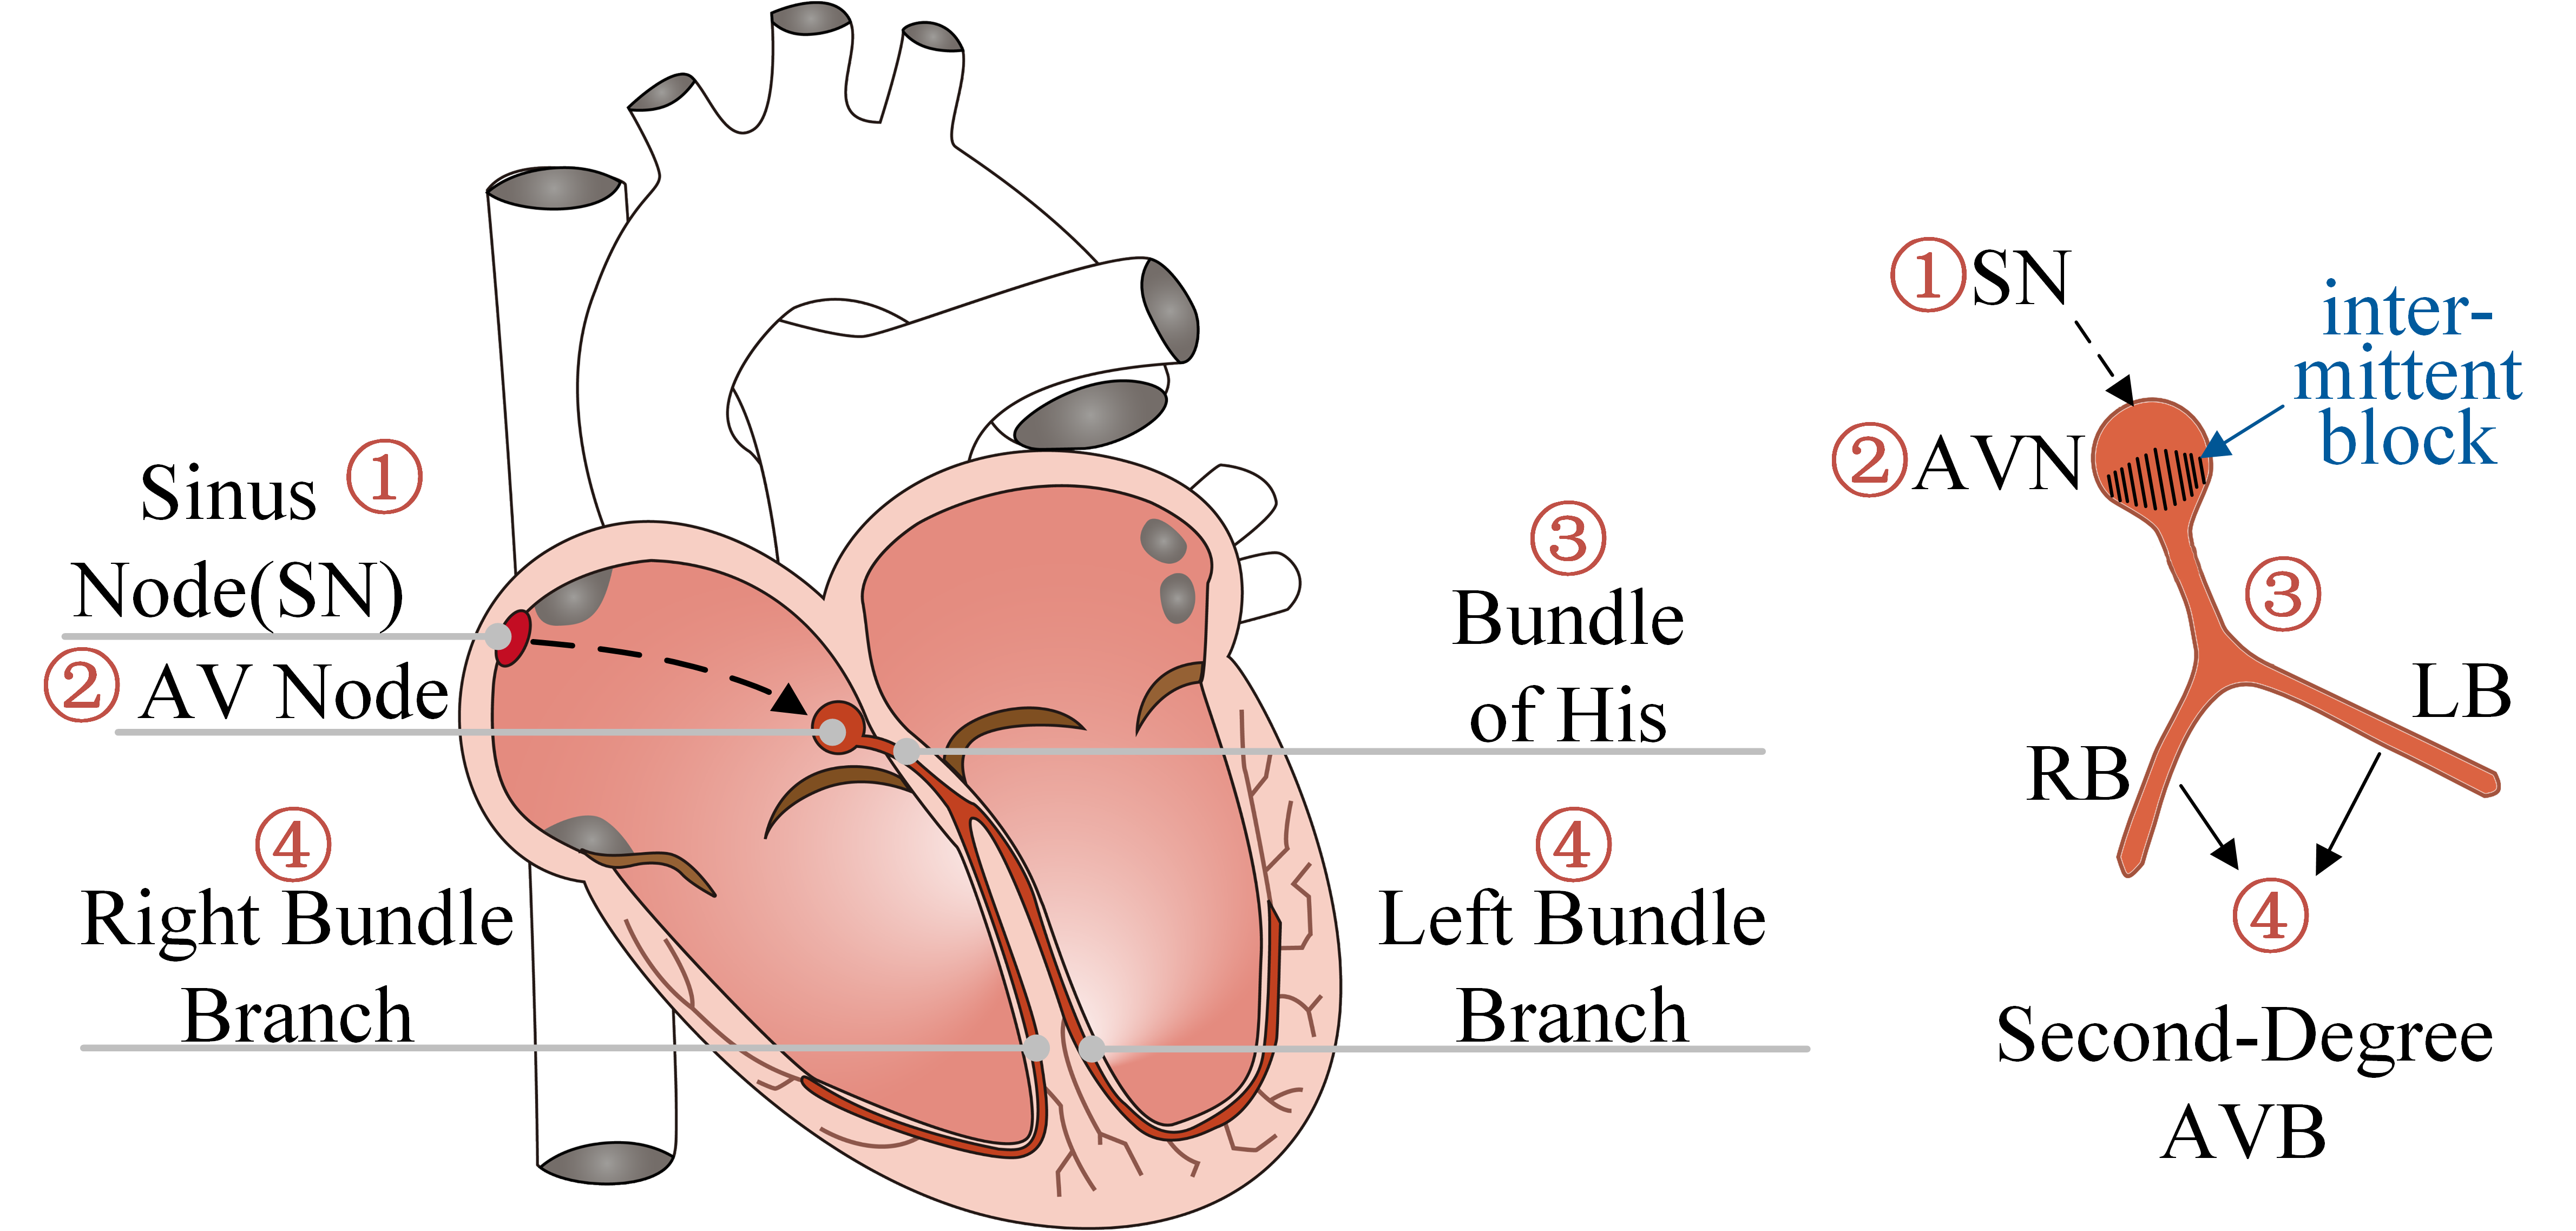
\includegraphics[width=0.7\linewidth]{Figure/AVB.png}
    \caption{图解第二重挑战：房室传导阻滞模型，P波后QRS波“丢失”，导致心动周期和信道状态的突然中断。}
\end{figure}

\subsection{本文的解决方案与主要学术贡献}
\begin{itemize}
    \item \textbf{技术方案：} 提出一种基于SRR的混合信号AGC架构，其核心是“预测-校正”双自由度（2-DOF）控制策略。
    \item \textbf{学术贡献：}
        \begin{enumerate}
            \item \textbf{理论创新：} 提出了无需ECG的心跳同步2-DOF主动补偿理论，将控制论中的前馈思想引入到生物信道自适应通信中。
            \item \textbf{方法学创新：} 建立了一个可编程的、能够高保真度复现临床病理动态的体外生物实验平台，为研究此类问题提供了可控、可重复的实验范式。
            \item \textbf{验证体系创新：} 构建了整合HIL仿真与体外实验的双路径定量评估框架，首次在学术上建立了从控制器瞬态响应指标到链路级通信可靠性的明确因果关联。
        \end{enumerate}
\end{itemize}

% ===================================================================
\section{方法学 (Methodology)}
% ===================================================================
\subsection{自适应接收机系统架构的硬件实现}
\begin{figure}[H]
    \centering
    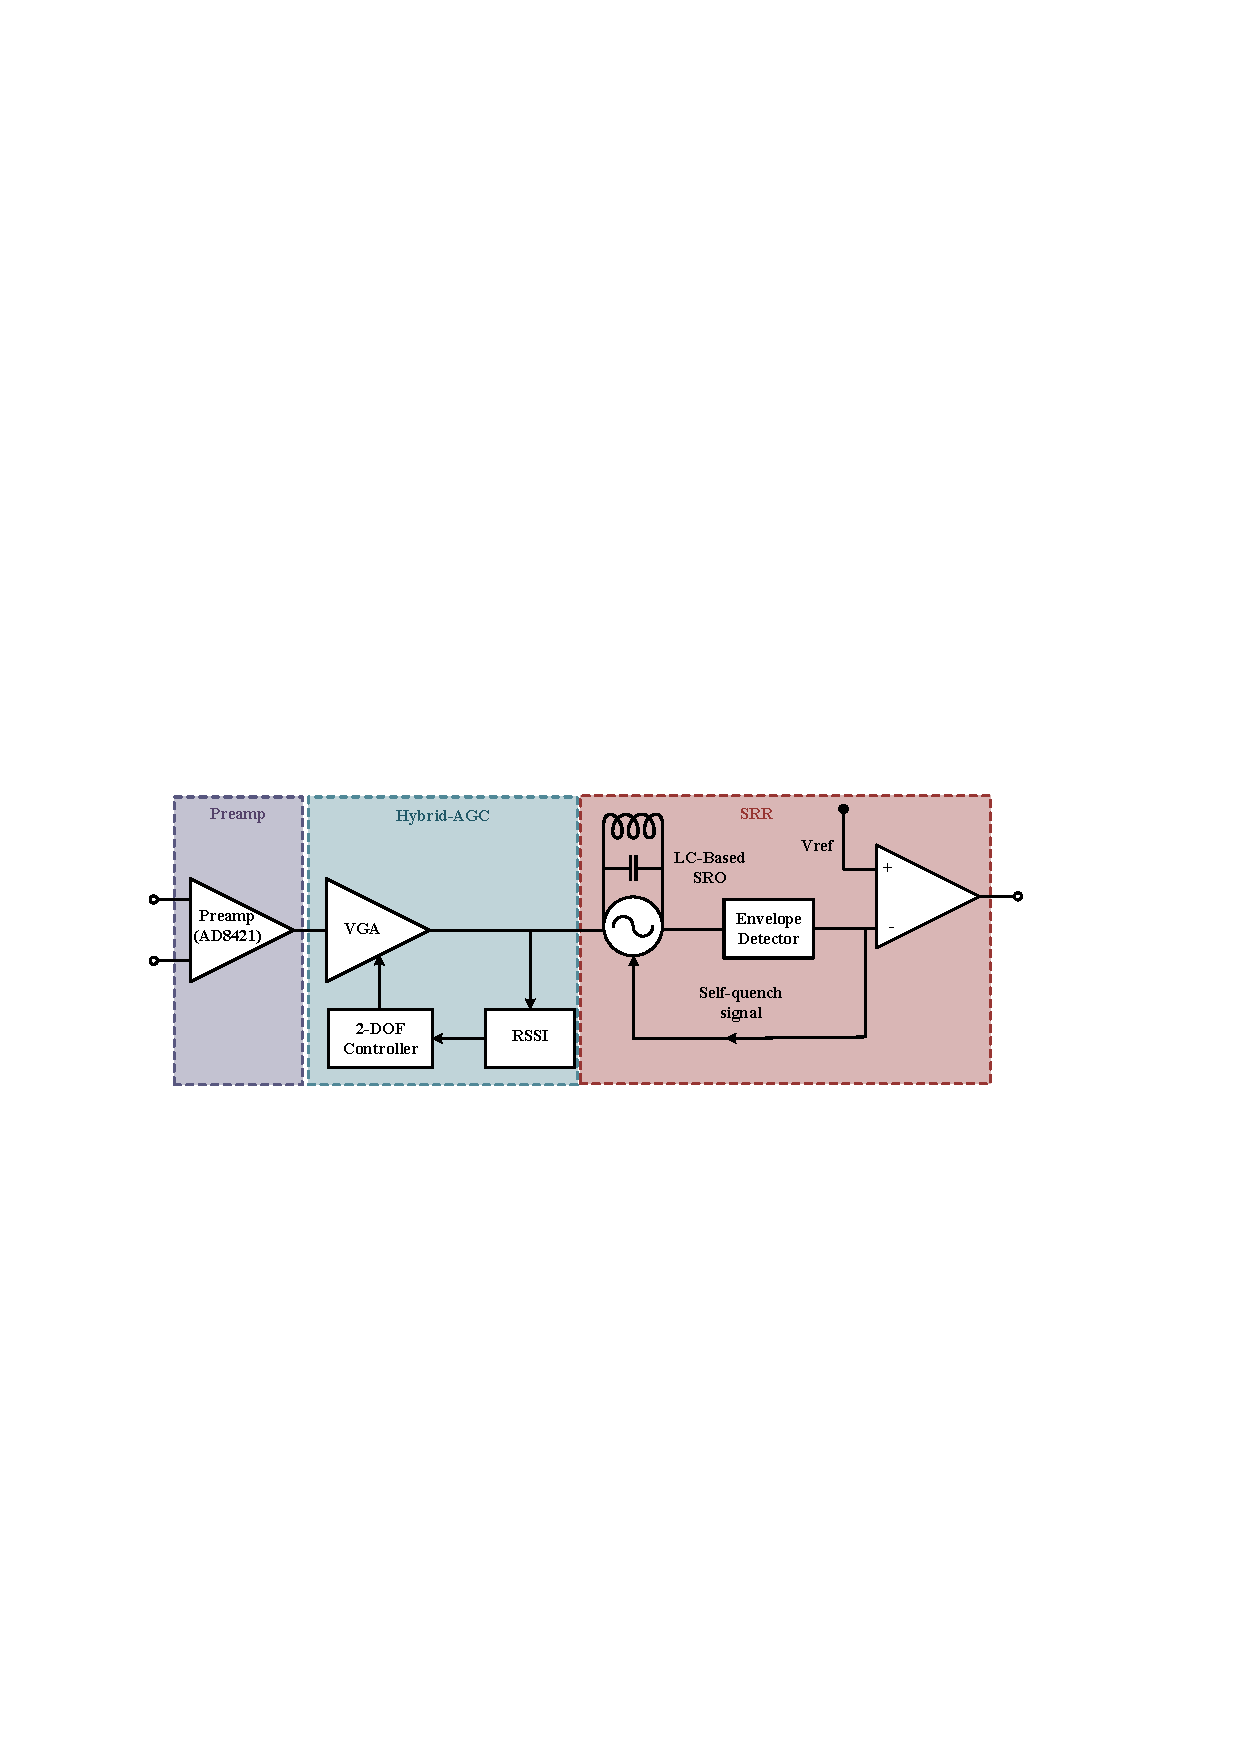
\includegraphics[width=0.5\linewidth]{Figure/framework}
    \caption{自适应接收机系统架构图，展示了从Preamp到VGA，再到RSSI和2-DOF数字控制核心，最终驱动SRR的完整信号与控制流。}
\end{figure}

\subsection{2-DOF 控制算法的形式化描述与实现细节}
\begin{itemize}
    \item \textbf{算法详述：} 提供了控制算法的伪代码（Algorithm 1），形式化地描述了：
        \begin{itemize}
            \item \textbf{心跳边界检测与峰值提取：} 如何从RSSI信号中自主识别心跳事件。
            \item \textbf{预测模型：} 采用指数移动平均（EMA）模型对下一个心跳的峰值信道增益进行预测。
            \item \textbf{前馈增益计算：} 基于预测值与目标值之差，计算前馈补偿量。
            \item \textbf{反馈回路：} 增量式PID控制器的差分方程实现，包括带滤波的微分项和抗积分饱和（Anti-Windup）机制。
            \item \textbf{输出合成与约束：} 前馈与反馈信号的合成，以及斜率限制（Slew-Rate Limiting）和饱和输出（Saturation）等硬件保护措施。
        \end{itemize}
\end{itemize}

\subsection{双路径实验验证体系的构建}
\begin{itemize}
    \item \textbf{高保真度生物仿真平台：} 详述了计算机控制的离体猪心灌注系统的构建细节，包括血泵的精确时序控制、血液模拟液的配方（匹配人体血液电导率），及其在模拟血液动力学方面的保真度验证。
    \item \textbf{评估协议的二元化设计：}
        \begin{enumerate}
            \item \textbf{瞬态响应评估 (HIL):} 目的是\keyterm{解耦控制器性能与生物样本的复杂性}。通过HIL仿真，注入标准的、可精确重复的阶跃干扰信号（5dB, 10dB, 15dB），从而在无生物噪声干扰下，定量测量控制器的建立时间（settling time）和最大偏差（maximum deviation）等关键动态指标。
            \item \textbf{通信可靠性评估 (Ex-vivo):} 目的是在\keyterm{最接近真实的、端到端的}条件下评估系统最终性能。在模拟的病理信道下，进行长序列伪随机二进制序列（PRBS）的传输，测量并对比不同方案（No-AGC, PID, 2-DOF）的最终误码率（BER）。
        \end{enumerate}
\end{itemize}
\begin{figure}[H]
    \centering
    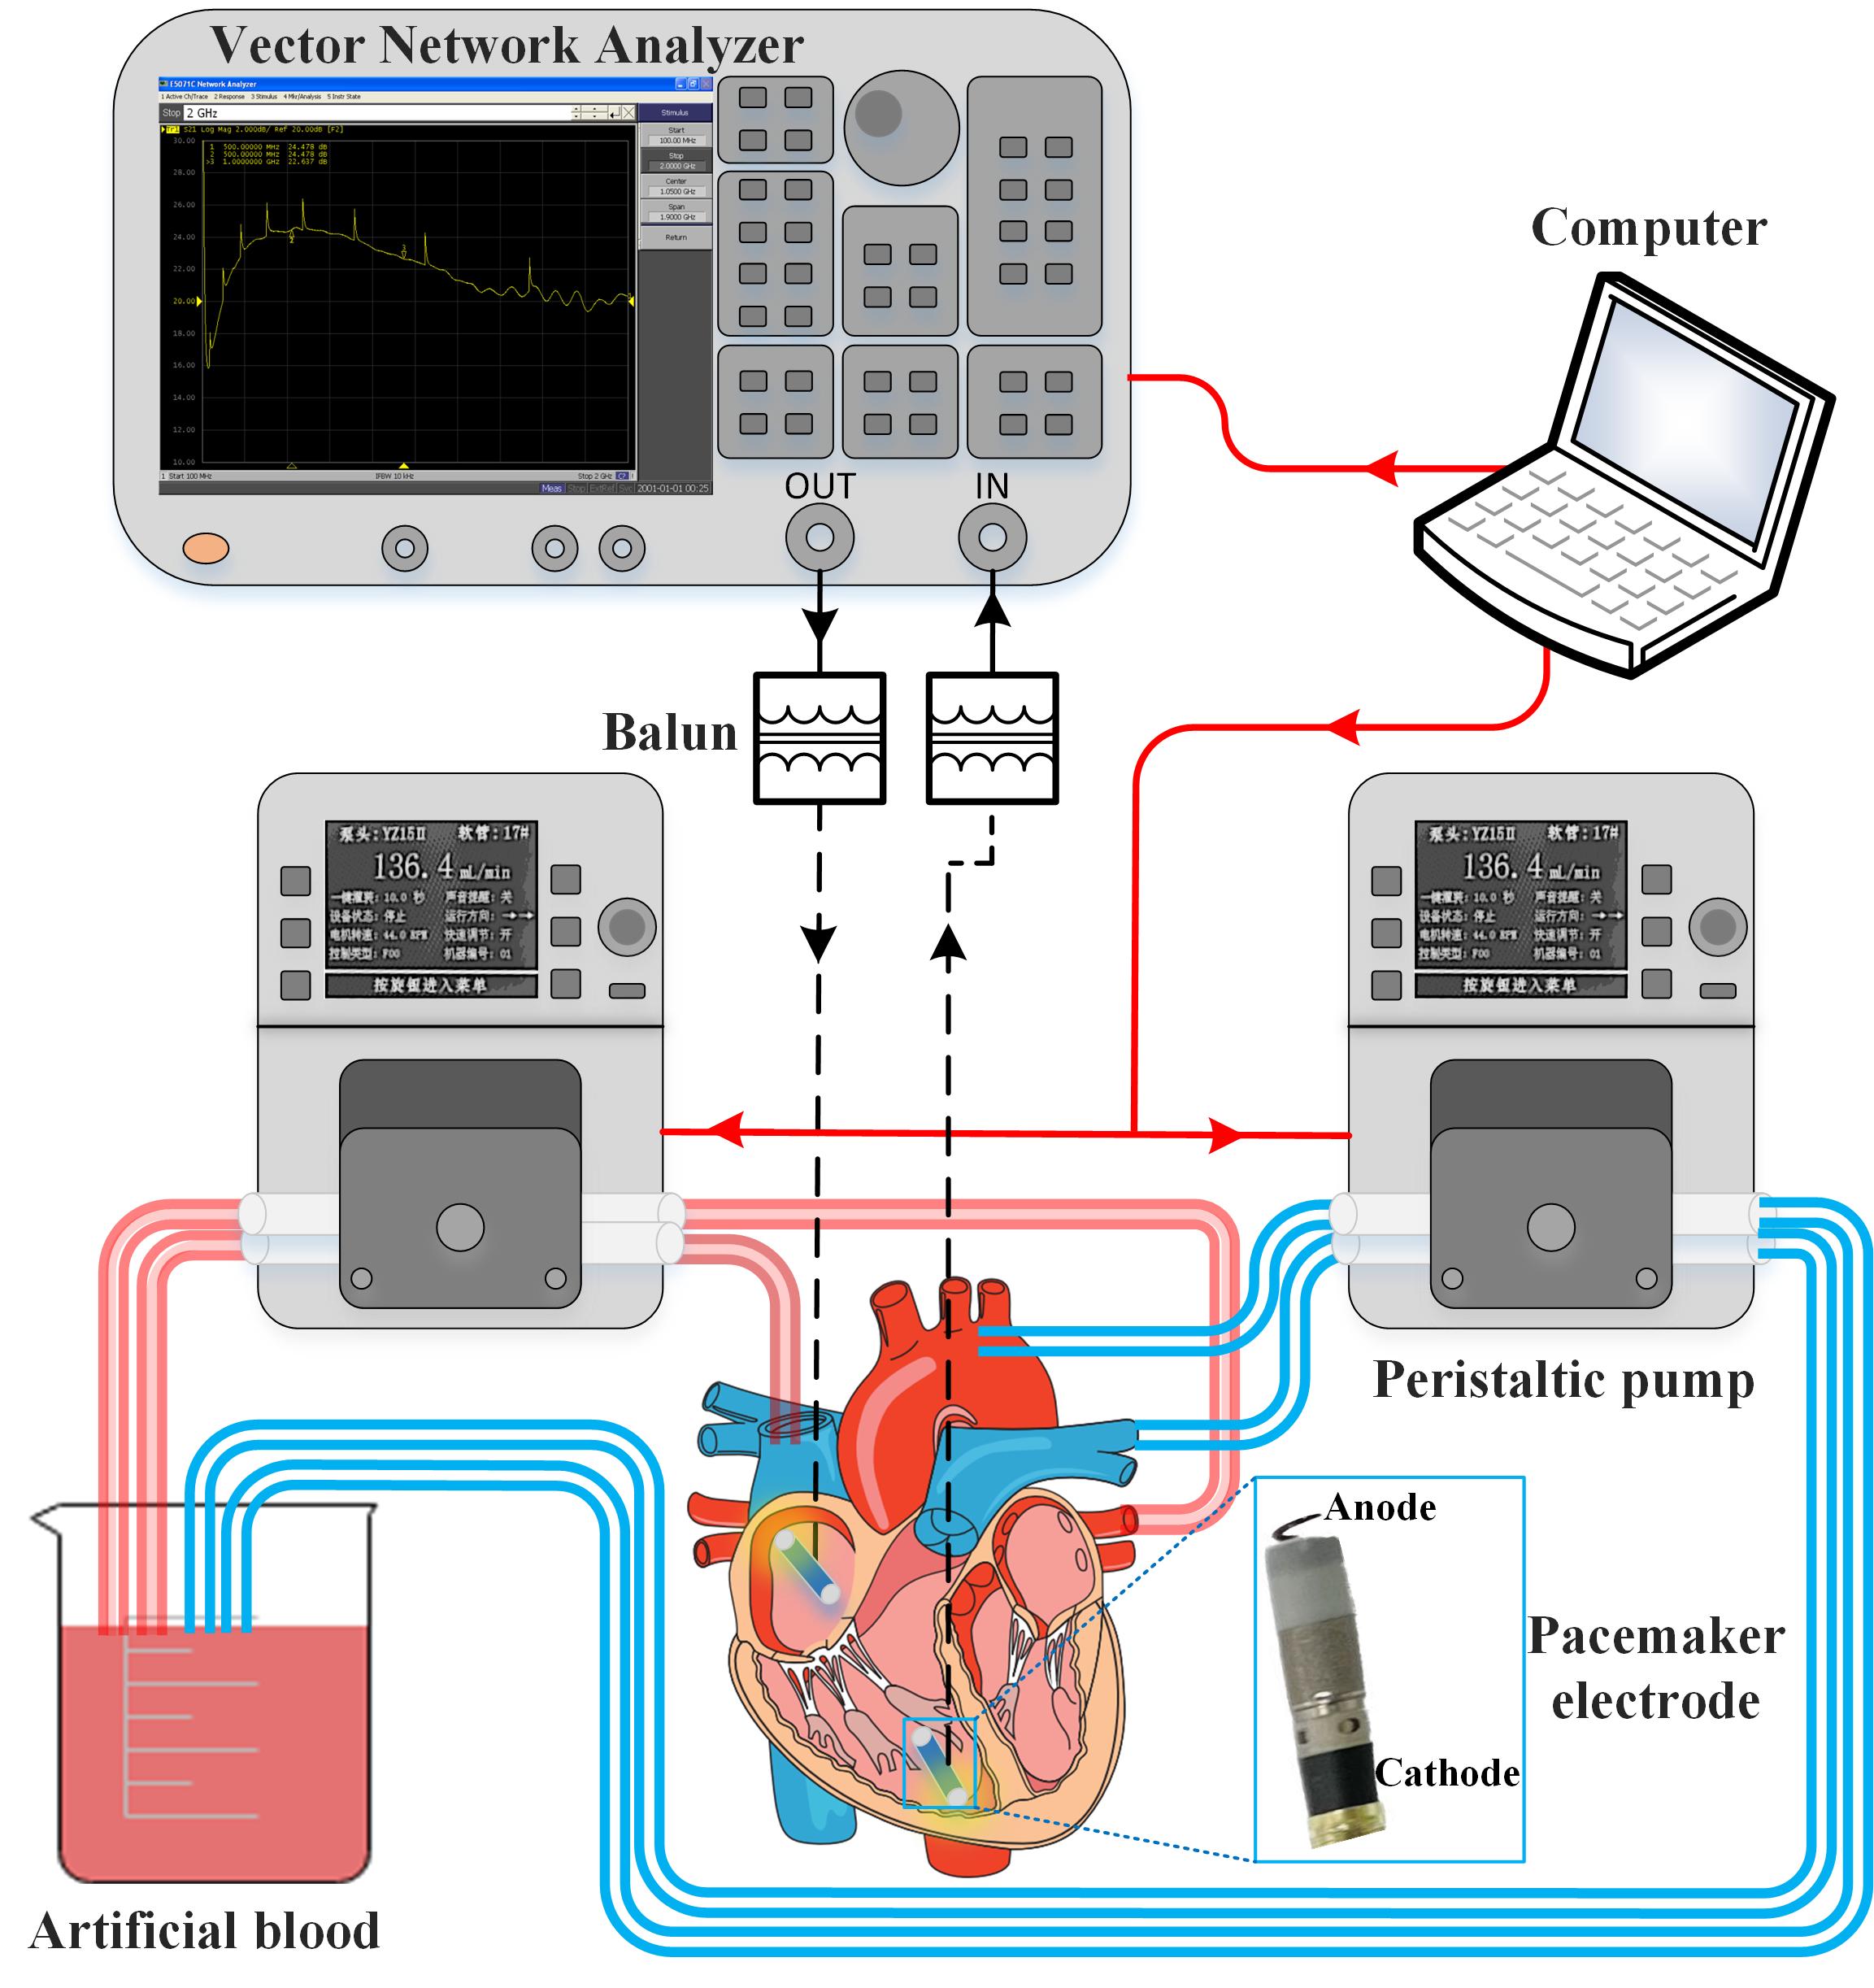
\includegraphics[width=0.5\linewidth]{Figure/measure_setup.png}
    \caption{实验验证平台与BER测试链路照片。}
\end{figure}






% ===================================================================
\section{实验结果与分析}
% ===================================================================
本部分通过构建一个四步的、层层递进的论证链，系统性地展示了从问题表征到最终方案验证的全过程。

\subsection{论证一：信道动态特性的定量表征——证明问题的客观存在与严峻性}
\begin{figure}[H]
    \centering
    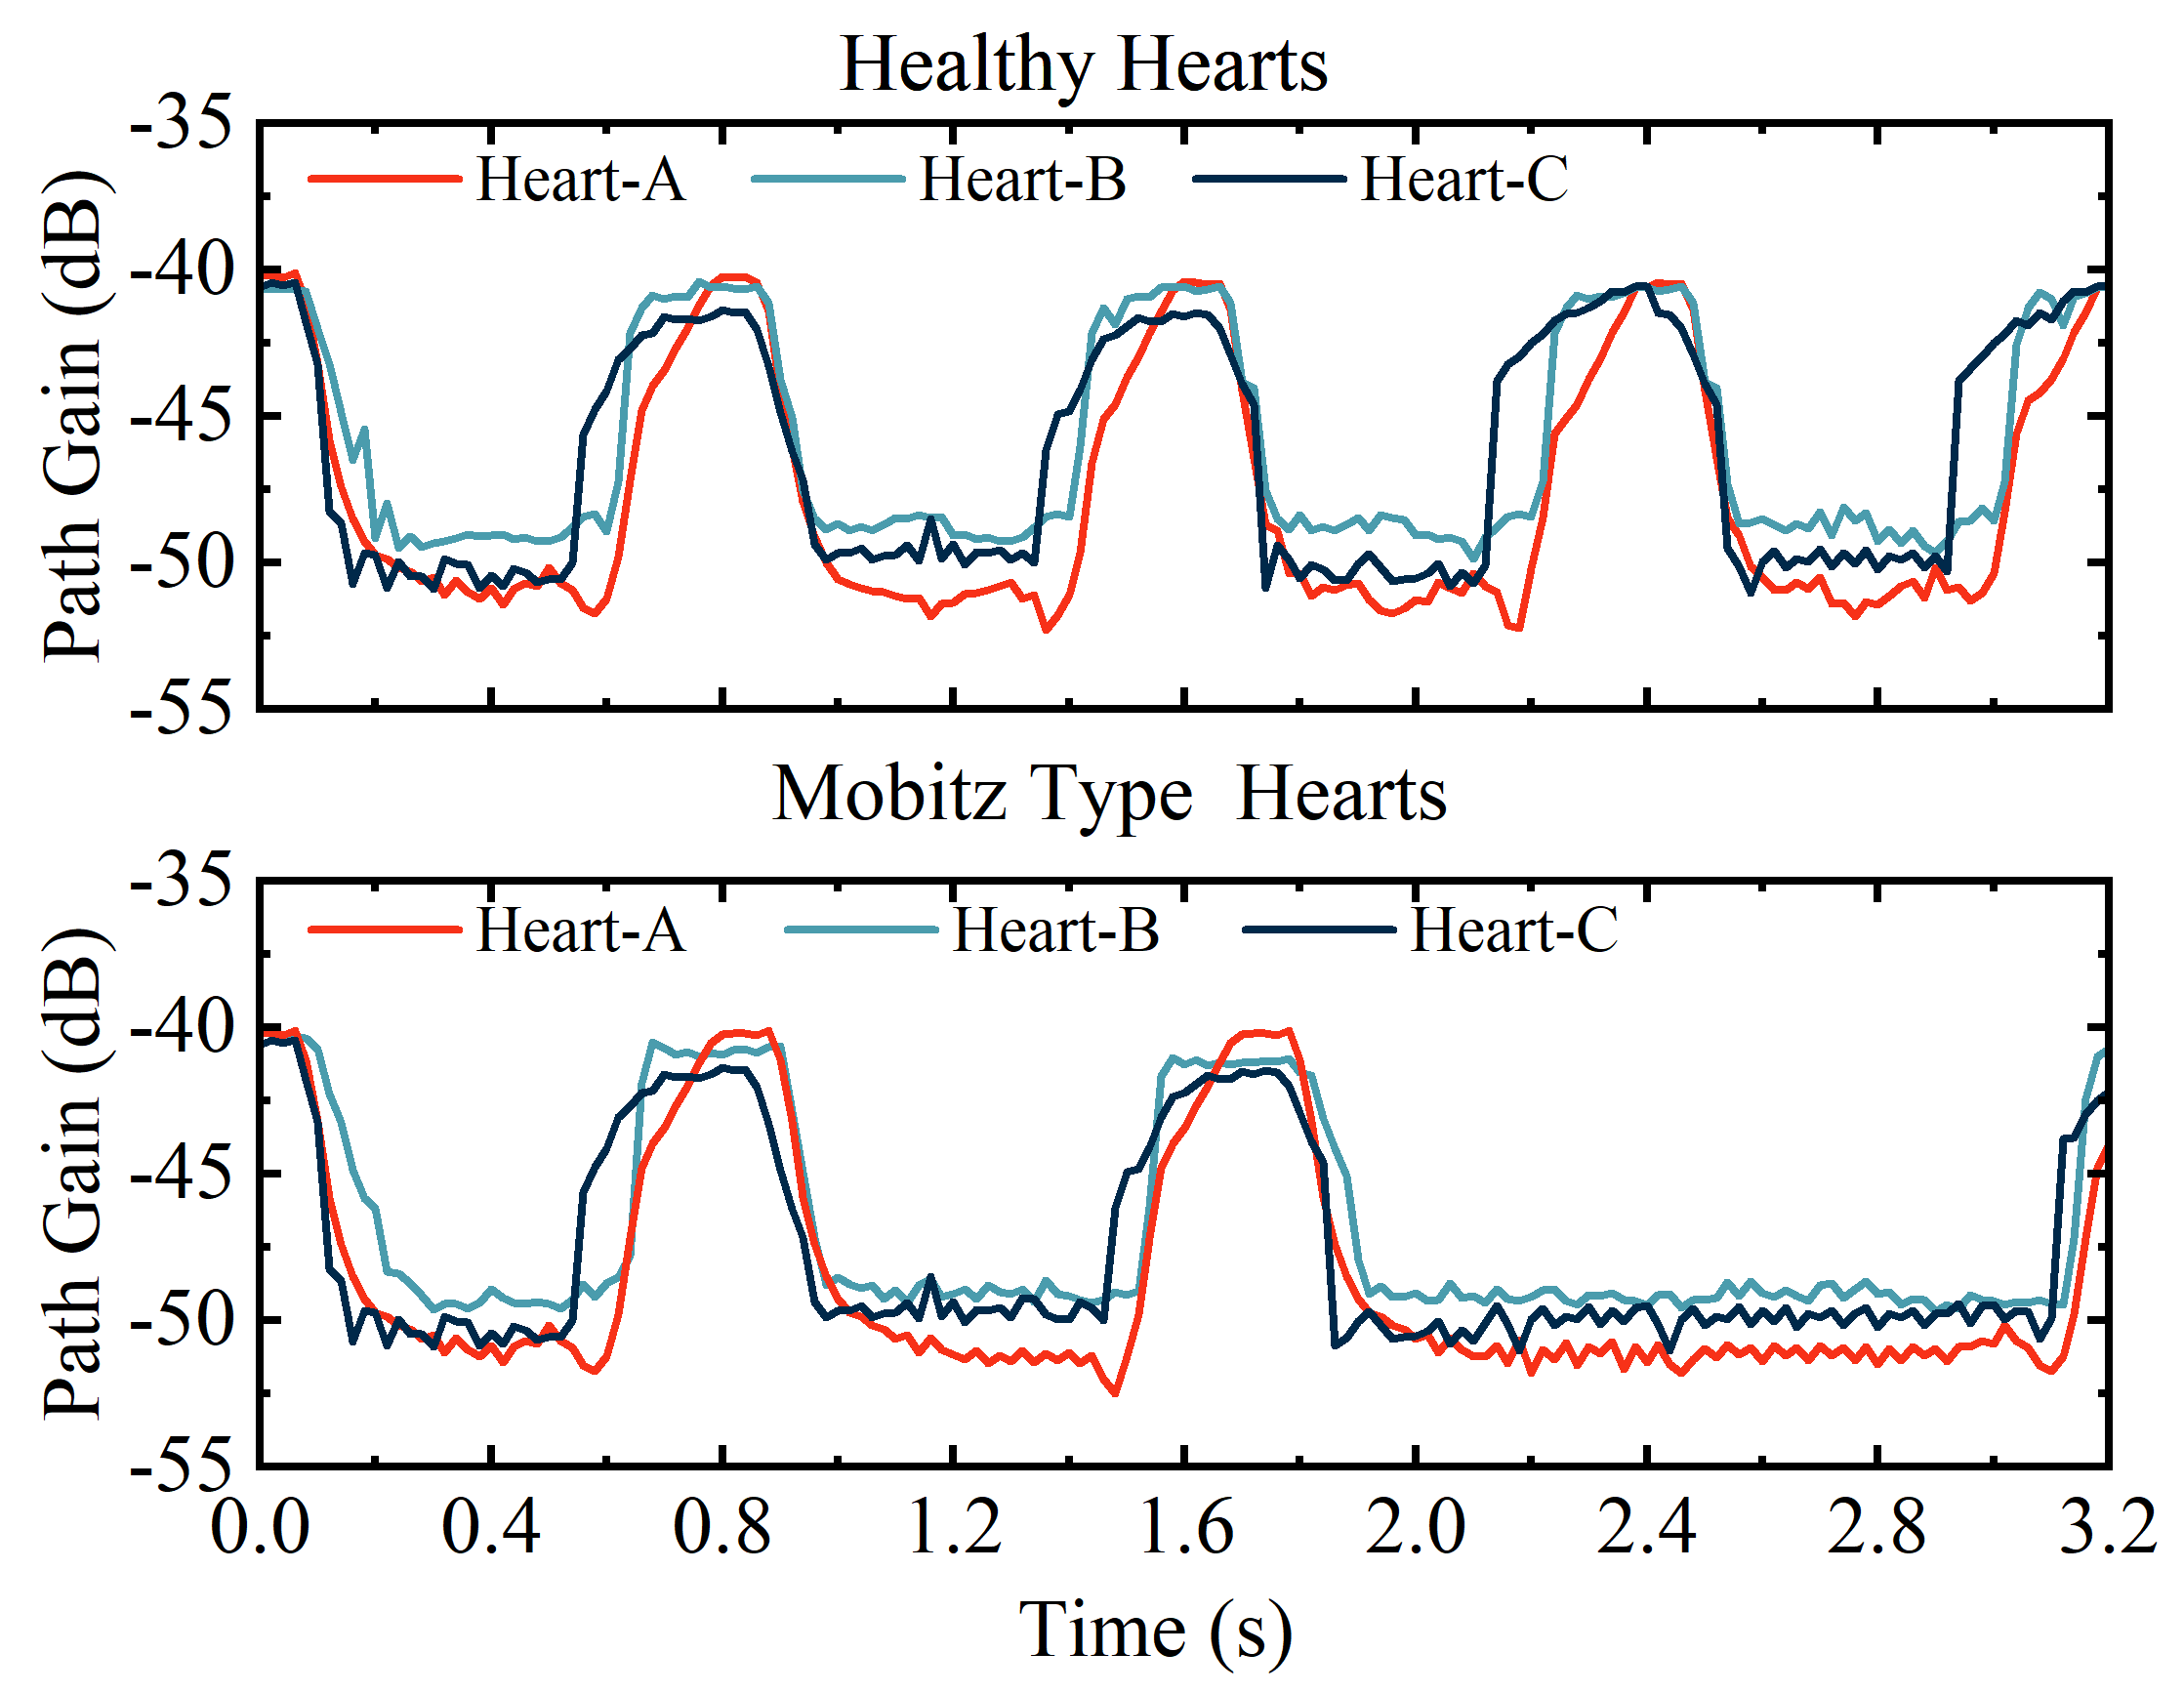
\includegraphics[width=0.5\linewidth]{Figure/signal_heart.png}
    \caption{信道增益的动态特性：(a) 健康心律下呈现高达10-15dB的周期性波动；(b) 病理心律下则转为不规则、更深度的突发性衰落。}
\end{figure}

\subsection{论证二：AGC系统的基础有效性验证——证明基础对策的必要性}
\begin{figure}[H]
    \centering
    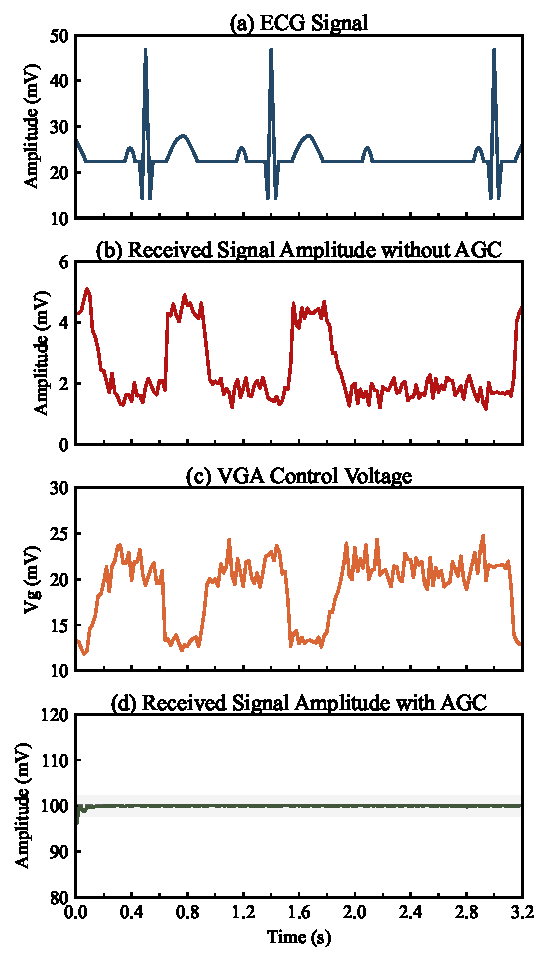
\includegraphics[width=0.7\linewidth]{Figure/agc}
    \caption{AGC系统的基本稳幅效果：与无控制的输入信号(b)相比，经AGC稳定后的信号(d)幅度被精确钳位在目标值，波动被抑制在1\%以内。}
\end{figure}

\subsection{论证三：2-DOF策略在瞬态响应上的优越性——证明本文方案的核心优势}
为了从控制论的根本层面验证2-DOF策略的先进性，我们通过硬件在环（HIL）测试，定量评估了其在面对信道阶跃干扰时的瞬态响应性能。这部分实验旨在证明，2-DOF的“预测”能力能够带来比纯反馈的PID更快的响应速度和更高的稳定性。

\begin{figure}[h!]
    \centering
    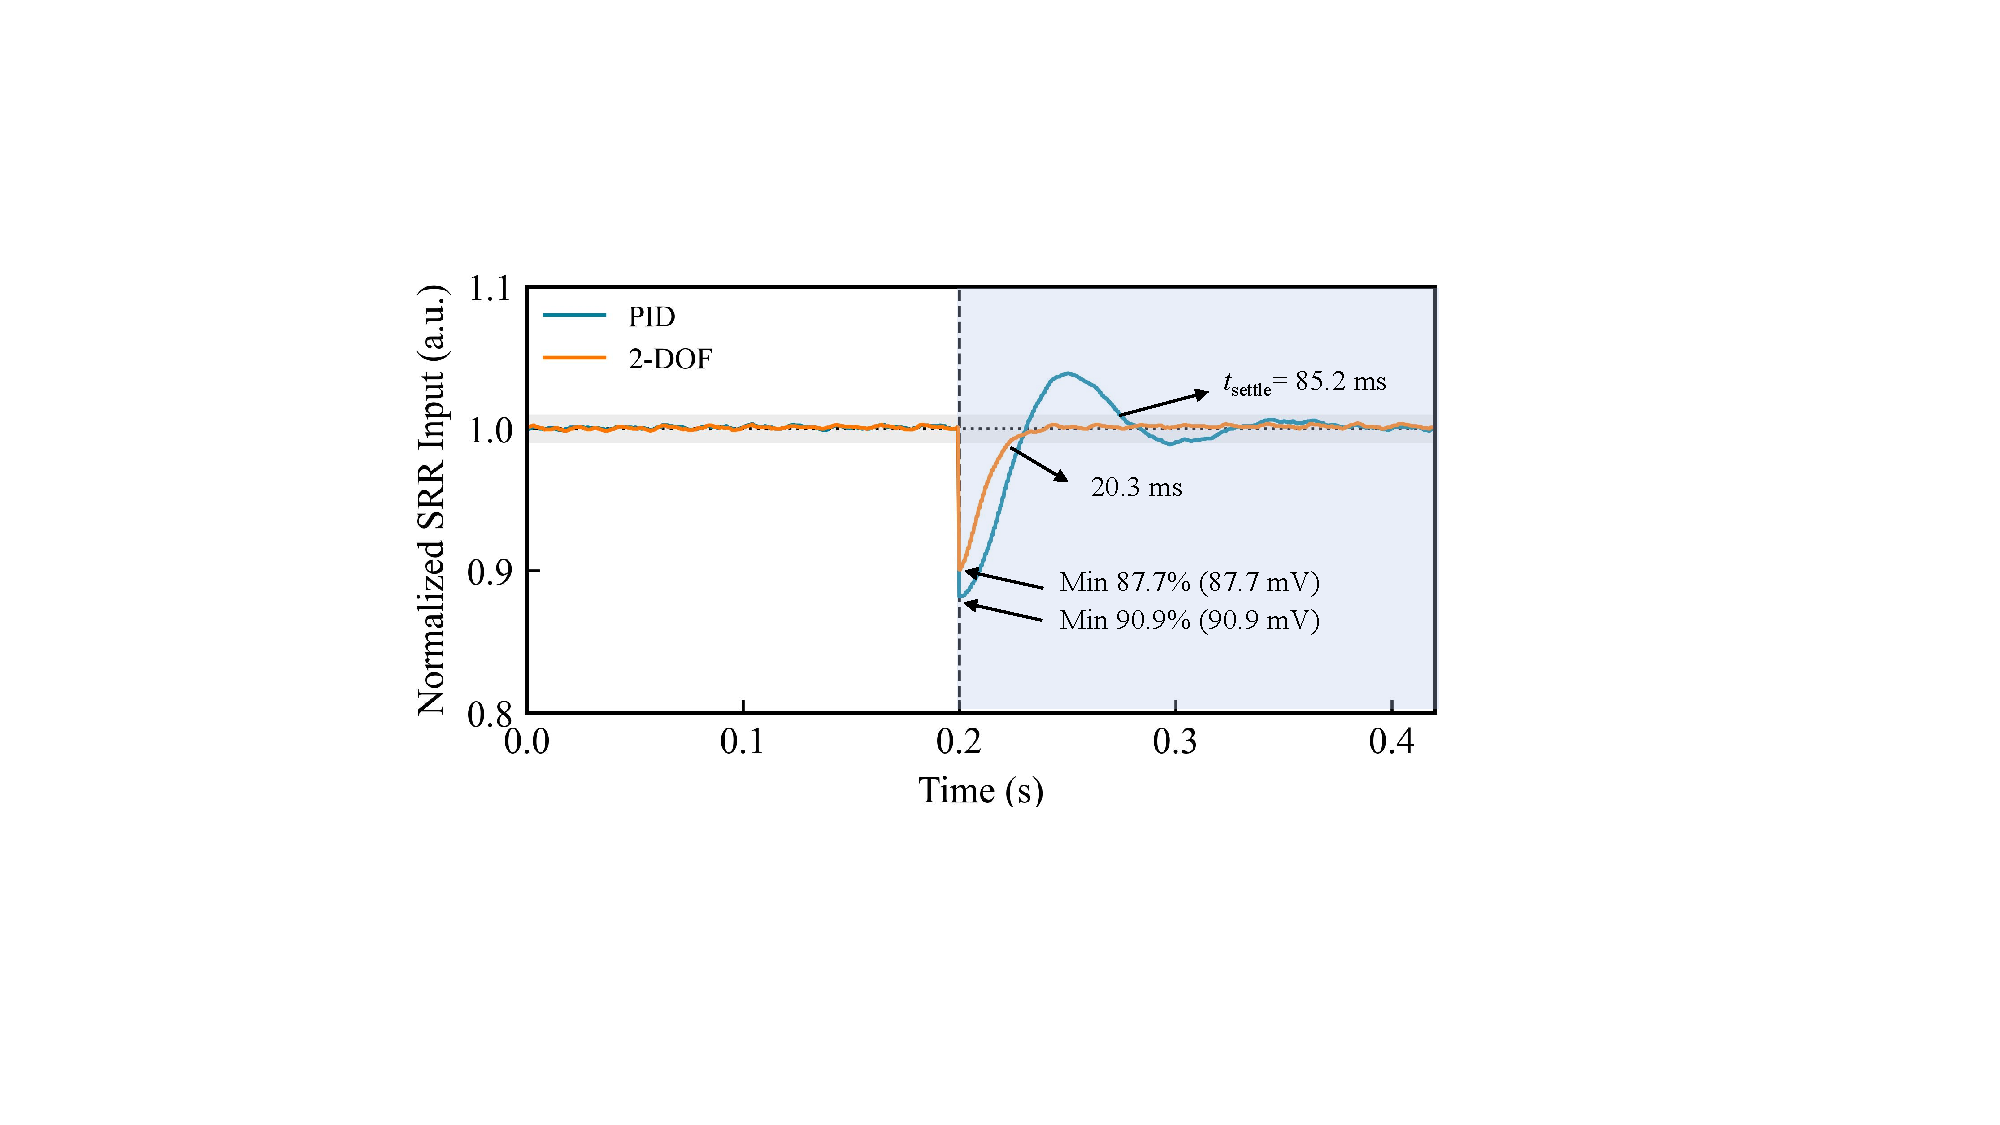
\includegraphics[width=0.5\linewidth]{Figure/step} % 这是您的 Fig. 10
    \caption{15dB信道阶跃下的单次瞬态响应对比。}
    \label{fig:step_single}
\end{figure}

如图 \ref{fig:step_single} 所示的单次典型事件中，2-DOF控制器（橙线）凭借其前馈预测能力，将建立时间从PID（蓝线）的85.2ms\textbf{缩短至20.3ms}（提速76\%），并显著减小了信号下冲幅度。

为了使这一结论具有统计学意义，我们进行了多组重复实验，结果如图 \ref{fig:step_bar} 所示。
\begin{figure}[h!]
    \centering
    % --- 这里插入您缺失的那张图 ---
    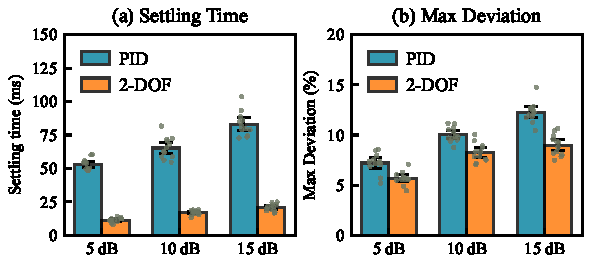
\includegraphics[width=0.5\linewidth]{Figure/R2_step_bar} % 假设您的文件名为 R2_step_bar.png
    \caption{瞬态性能指标的定量统计对比。}
    \label{fig:step_bar}
\end{figure}

该统计结果无可辩驳地证明了2-DOF架构的全面优势：
\begin{itemize}
    \item \textbf{在响应速度上 (Settling Time):} 无论是在5dB, 10dB, 还是15dB的阶跃干扰下，2-DOF的建立时间始终比PID快约\textbf{4倍}，平均降幅达到76\%。
    \item \textbf{在稳定性上 (Max Deviation):} 2-DOF的最大信号偏差也 consistently 比PID小20-26\%。
\end{itemize}


\subsection{论证四：端到端通信可靠性的最终验证——展示最终成果}
\begin{figure}[H]
    \centering
    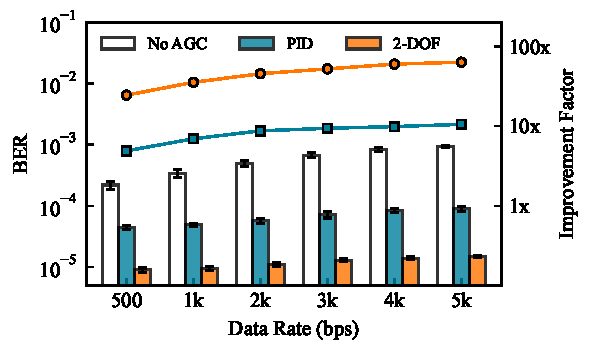
\includegraphics[width=0.5\linewidth]{Figure/ber}
    \caption{BER性能对比。左轴：误码率；右轴：相对No-AGC的性能提升因子。}
\end{figure}
\begin{itemize}
    \item \textbf{主要结论1 (绝对性能):} 在所有测试数据率下，2-DOF架构（橙色柱）均实现了最低的误码率，证明了其在绝对性能上的优越性。
    \item \textbf{主要结论2 (趋势与鲁棒性):} 2-DOF架构的性能优势（橙色线）\textbf{随数据率的增加而愈发显著}，其性能提升因子从500bps下的约24倍增长至5kbps下的超过63倍。这强有力地证明了其对高速通信中码间干扰（ISI）的强大抑制能力，这正是其优越瞬态响应性能所带来的直接成果。
\end{itemize}






\textbf{结论：} 这一系列的瞬态响应数据，为2-DOF控制器最终能够在高速通信中（论证四）表现出更强鲁棒性，提供了坚实的底层物理机制支撑。它的快速稳定能力，是抑制码间干扰的关键。












% ===================================================================
\section{讨论与结论 (Discussion \& Conclusion) - 成果的总结、定位与展望}
% ===================================================================
\subsection{核心科学贡献的重申}
\begin{itemize}
    \item 本研究的核心贡献在于，针对病理性心律这一动态、非预测性信道，提出并验证了一种有效的自适应通信方案，实现了从传统的“被动适应”到“主动预测”的设计哲学转变。
\end{itemize}

\subsection{与相关工作的比较与定位}
\begin{itemize}
    \item 依据性能对比表（Table II），明确指出本工作与相关研究的区别：先前工作主要关注静态信道表征、调制方案或低功耗电路实现，而本工作则首次系统性地解决了\keyterm{“病理信道稳健性”}这一关键的临床应用问题，并提供了有效的\keyterm{自适应增益补偿}方案，填补了现有技术的空白。
\end{itemize}


\subsection{与相关工作的比较与定位：凸显本研究的独特性}
本研究的核心创新点，可以通过与领域内相关先进原型机的多维度对比得到最清晰的体现。如下表所示，本工作在研究焦点和技术实现上，填补了现有研究的关键空白。

\begin{table}[H]
\centering
\caption{与相关接收机原型机的性能对比}
\label{tab:comparison_summary}
\resizebox{\textwidth}{!}{%
\begin{tabular}{l l l l l l}
\toprule
\textbf{Metric} & \textbf{Bereuter et al. [25]} & \textbf{Ryser et al. [24]} & \textbf{Khaleghi et al. [20]} & \textbf{Yuk et al. [38]} & \textbf{This Work} \\
\midrule
Primary focus & In-vivo channel char. & Modulation scheme & Broadband channel & Low-power IC & \textbf{Pathological channel} \\
& & analysis & modeling & & \textbf{robustness} \\
\addlinespace
Measurement Type & In-vivo & Ex-vivo & Ex-vivo & In-vivo/Ex-vivo & Ex-vivo \\
\addlinespace
Frequency [MHz] & 1 & 1.5 & 0.01-10 & DC-20 & 1 \\
\addlinespace
Receiver Power [mW] & $>$465 & 152 & 230 & \textbf{0.062} & 268 \\
\addlinespace
Technology & Discrete comp. & Discrete comp. & Discrete comp. & \textbf{110nm CMOS} & Discrete comp. \\
\midrule
NSR Dynamics & $\times$ & $\times$ & $\times$ & $\times$ & \huge\checkmark \\
\addlinespace
Pathological Dynamics & $\times$ & $\times$ & $\times$ & $\times$ & \huge\checkmark \\
\addlinespace
Adaptive Gain Comp. & $\times$ & $\times$ & $\times$ & $\times$ & \huge\checkmark \\
\bottomrule
\end{tabular}
}
\end{table}




\subsection{研究的局限性与未来展望}
\begin{itemize}
    \item \textbf{承认局限性：} 坦诚当前体外研究无法完全模拟所有体内生理因素（如自主神经调节、呼吸耦合、长期电极-组织界面变化等）。
    \item \textbf{展望未来工作：} 明确了后续的研究路径：1) 将当前的分立元件原型进行\keyterm{CMOS集成电路化}，以满足植入式设备的体积与功耗要求；2) 开展覆盖更多病理类型和更长周期的\keyterm{在体大型动物实验}，以最终验证该技术的临床转化潜力。
\end{itemize}

\subsection{总结性陈述 (Concluding Remarks)}
\begin{itemize}
    \item 所提出的心跳同步2-DOF自适应接收机架构，为下一代要求高可靠性、并需在严苛生物环境中稳健运行的网络化植入式医疗设备，提供了一套经过系统性验证的关键使能技术与可推广的设计范式。
\end{itemize}

\end{document}